% Intended LaTeX compiler: pdflatex
\documentclass[UTF8]{ctexart}
\documentclass[11pt]{article}
\usepackage[utf8]{inputenc}
\usepackage[T1]{fontenc}
\usepackage{graphicx}
\usepackage{grffile}
\usepackage{longtable}
\usepackage{wrapfig}
\usepackage{rotating}
\usepackage[normalem]{ulem}
\usepackage{amsmath}
\usepackage{textcomp}
\usepackage{amssymb}
\usepackage{capt-of}
\usepackage{hyperref}
\author{孙其鲁}
\date{\today}
\title{软件安全实验报告}
\hypersetup{
 pdfauthor={孙其鲁},
 pdftitle={软件安全实验报告},
 pdfkeywords={},
 pdfsubject={},
 pdfcreator={Emacs 27.2 (Org mode 9.4.4)}, 
 pdflang={English}}
\begin{document}

\maketitle

\section*{实验一安装并使用EMACS}
\label{sec:org7711d16}
\subsection*{一、实验要求}
\label{sec:org262c9d3}
\begin{itemize}
\item 在Windows 10 下安装EMACS程序
\item 安装一个EVIL插件,并切换到evil-mode模式
\item 熟悉 EMACS 的编辑命令
\item 在书写实验报告时,附带必要实验屏幕截图
\end{itemize}
\subsection*{二、实验步骤}
\label{sec:org7bd38d5}
\subsubsection*{1.熟悉基本按键}
\label{sec:orged5e056}
\texttt{C-x} 表示 \texttt{Ctrl+x} , \texttt{M-x} 表示 \texttt{Alt + x} , \texttt{S-Tab} 表示 \texttt{Shift + Tab} , \texttt{RET} 表示按下 Enter 键。
\subsubsection*{2.将按键 \texttt{Esc} 与按键 \texttt{CapsLock} 相互交换}
\label{sec:org1912120}
\begin{itemize}
\item 1.打开注册表编辑器.
\label{sec:org08c1376}
\begin{center}
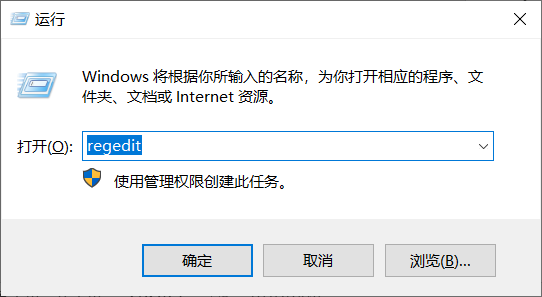
\includegraphics[width=.9\linewidth]{image/1.png}
\end{center}
\item 2.找到HKEY\_LOCAL\_MACHINE\SYSTEM\CurrentControlSet\Control\Keyboard Layout,在右边窗口右击,新建->新建二进制值,选中新建对象,右击修改。将数值名称改为Scancode Map。将数值数据改为hex:00,00,00,00,00,00,00,00,03,00,00,00,3a,00,01,00,01,00,3a,00,00,00,00,00保存即可。
\label{sec:org39afecb}
\begin{center}
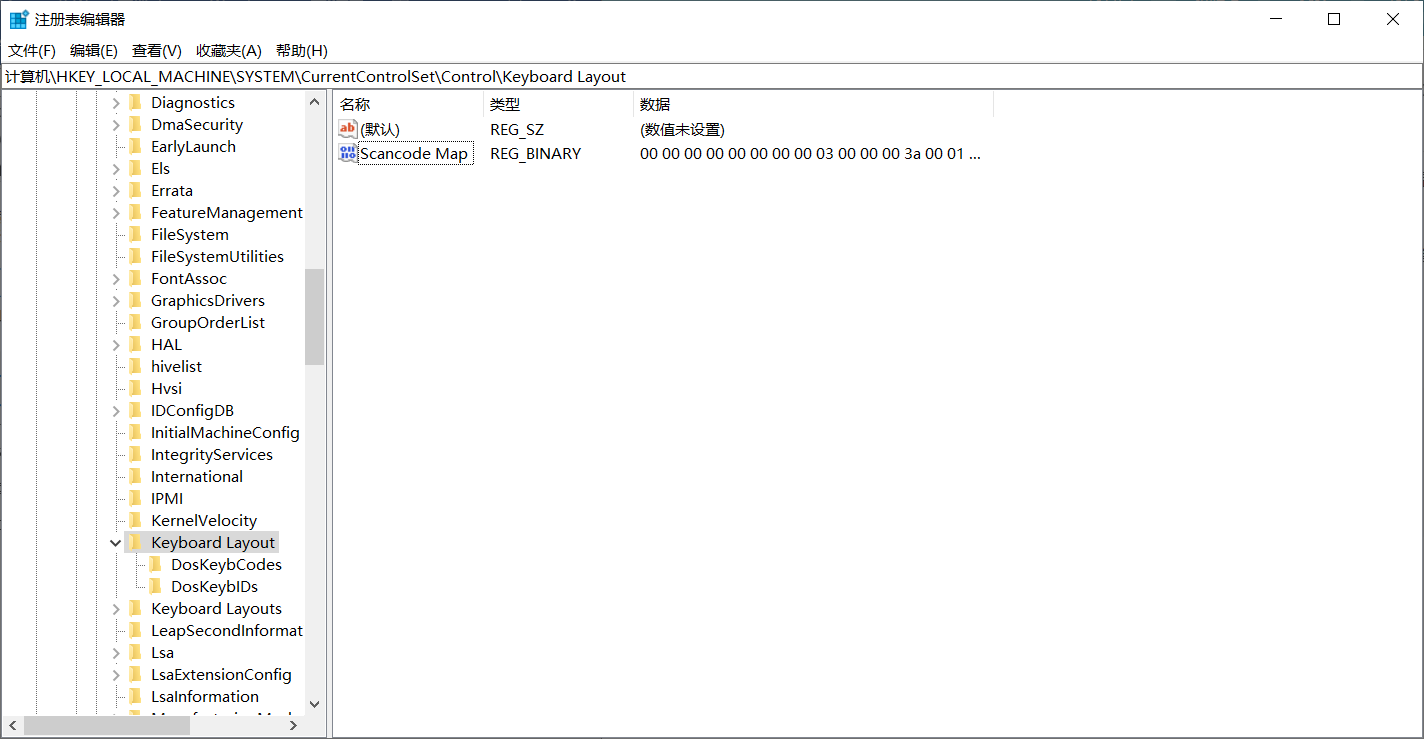
\includegraphics[width=.9\linewidth]{image/2.png}
\end{center}
\end{itemize}
\subsubsection*{3.修改自定义HOME}
\label{sec:org4e3c6bd}
\begin{itemize}
\item 1.在 \texttt{share\textbackslash{}emacs\textbackslash{}site-lisp} 下创建 \texttt{site-start.el} 文件,并写下如下内容
\label{sec:org0ab9eb5}
\begin{verbatim}
(defun set-home-dir (dir)
(setenv "HOME" dir)
(message (format "HOME location is %s" (getenv "HOME")))) 
(set-home-dir "D:/EmacsDocuments")
\end{verbatim}
\item 2.在 \texttt{E:\textbackslash{}EmacsDocuments} 下创建 \texttt{.emacs.d} 文件夹,HOME修改成功
\label{sec:org29cc1e4}
\end{itemize}
\subsubsection*{4.在Windows 10 安装EMACS基本步骤}
\label{sec:org2653839}
\begin{itemize}
\item 1. 到 \href{http://www.gnu.org/software/emacs/}{GNU Emacs} 的官网下载 Emacs 软件,选择 \href{https://www.gnu.org/software/emacs/download.html\#nonfree}{Windows} ,然后选择 \href{http://ftp.gnu.org/gnu/emacs/windows/}{main GNU FTP} 。在 FTP 服务器上根据机器是 32 位还是 64 位操作系统选择以 \texttt{.zip} 结尾的软件。
\label{sec:org23cd40f}
\begin{center}
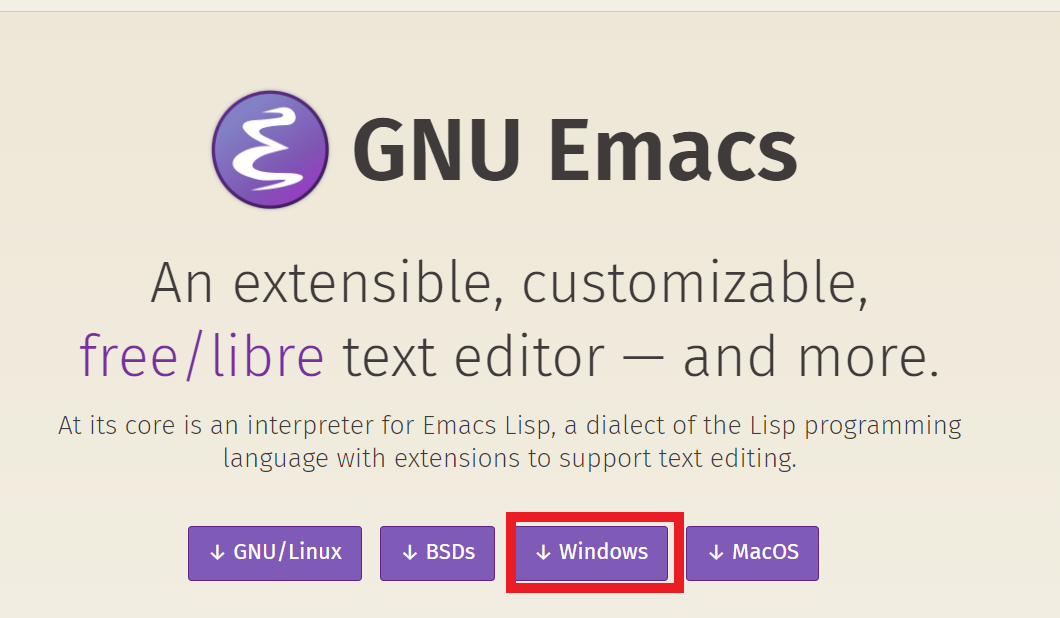
\includegraphics[width=.9\linewidth]{image/3.png}
\end{center}
\begin{center}
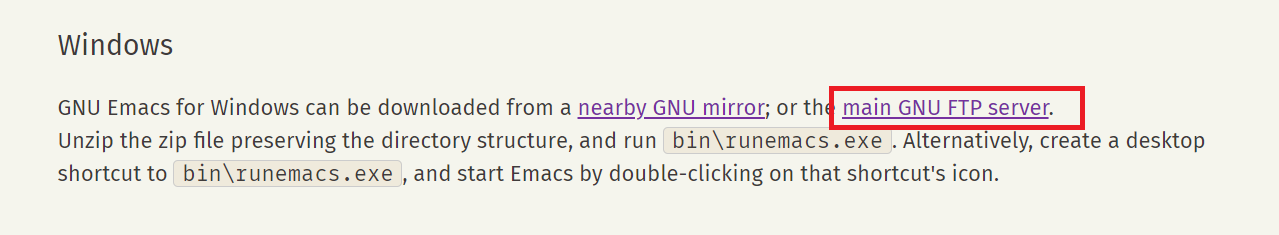
\includegraphics[width=.9\linewidth]{image/4.png}
\end{center}
\begin{center}
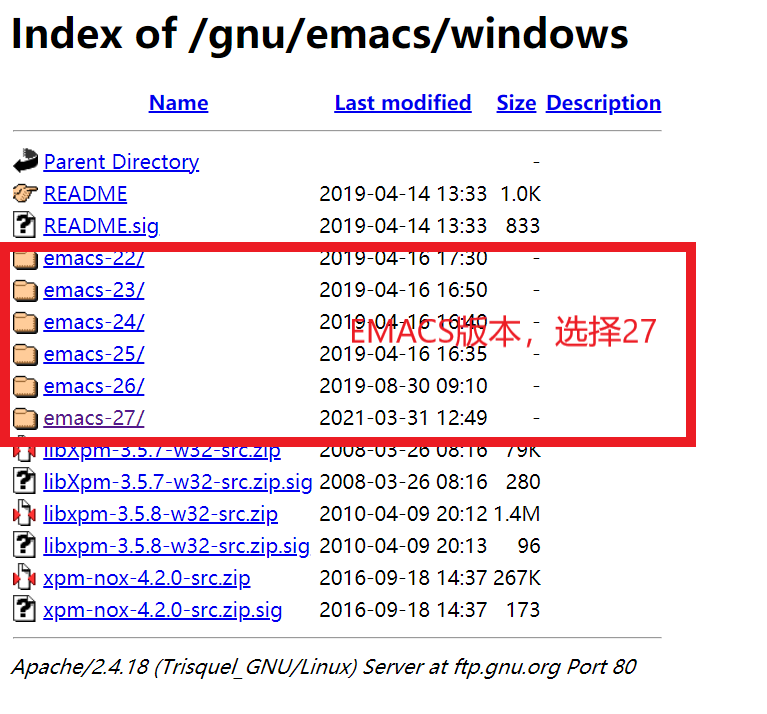
\includegraphics[width=.9\linewidth]{image/5.png}
\end{center}
\begin{center}
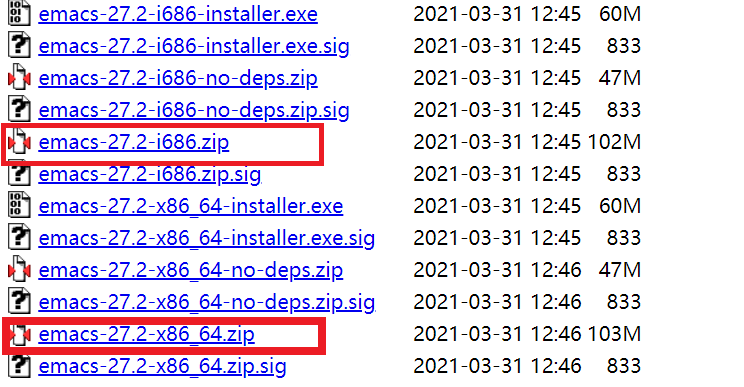
\includegraphics[width=.9\linewidth]{image/6.png}
\end{center}
\item 2. 找到解压缩文件中的 \texttt{emacs/bin/runemacs.exe} 并发送到桌面,更改名称为 \texttt{emacs} ,只有在 \texttt{runemacs.exe} 运行时不会弹出 "命令行窗口" 对话框。
\label{sec:orgb4f12ec}
\begin{center}
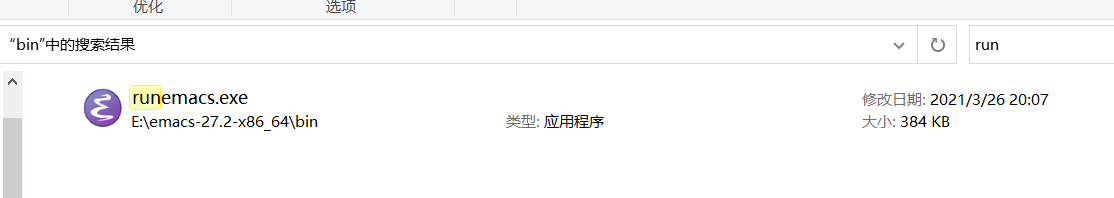
\includegraphics[width=.9\linewidth]{image/7.png}
\end{center}
\item 3. 在 \texttt{D:\textbackslash{}Emacs\textbackslash{}Documents} 下创建 \texttt{init.el} 文件。最基本的操作是连接 MEPLA 插件库,因此学会阅读 \href{https://melpa.org/\#/getting-started}{MEPLA} 帮助文档的内容。
\label{sec:org57d64bb}
\begin{center}
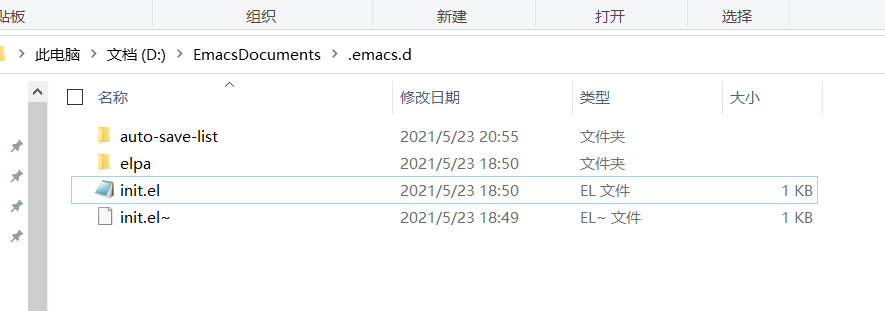
\includegraphics[width=.9\linewidth]{image/8.png}
\end{center}
\begin{itemize}
\item 打开 MEPLA 初学者必须查看的 \href{https://melpa.org/\#/getting-started}{START} 页面。将以下内容复制粘贴到 \texttt{init.el} 文件中。
\begin{verbatim}
:(require 'package)
;; 此为 MEPLA 官方插件服务器地址,如果国内访问速度慢也可访问清华大学的MEPLA服务器镜像地址
(add-to-list 'package-archives '("melpa" . "https://melpa.org/packages/") t)
(package-initialize)
\end{verbatim}
\end{itemize}
\begin{center}
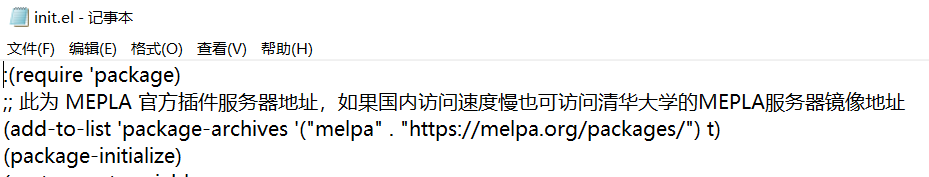
\includegraphics[width=.9\linewidth]{image/9.png}
\end{center}
\begin{itemize}
\item 运行 \texttt{M-x package-refresh-contents} 刷新插件服务器内容;运行 \texttt{M-x package-install RET} 后输入 \texttt{M-x evil-org} 安装此插件。
\begin{center}
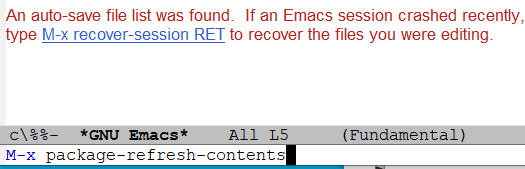
\includegraphics[width=.9\linewidth]{image/10.png}
\end{center}
\begin{center}
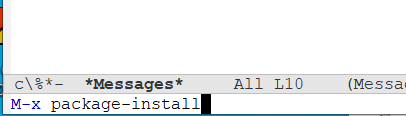
\includegraphics[width=.9\linewidth]{image/11.png}
\end{center}
\begin{center}
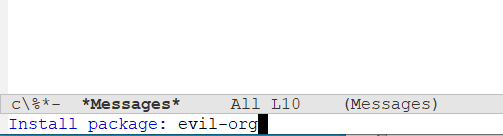
\includegraphics[width=.9\linewidth]{image/12.png}
\end{center}
\item 以上述方法安装 \texttt{which-key} 插件,该插件安装成功后, 当输入 \texttt{M-x package} 时会看到 EMACS 能弹出 POPWINDOWS 提示窗口,非常方便。
\end{itemize}

\item 4. 切换到 EVIL-MODE 模式。输入命令 \texttt{M-x evil-mode} 切换到 EVIL 模式,此时将会以 VIM 的按键方式移动鼠标。测试在 NORMAL 模式下,按下 \texttt{hjkl} 键鼠标是否上下移动。
\label{sec:orgcf854e5}
\begin{center}
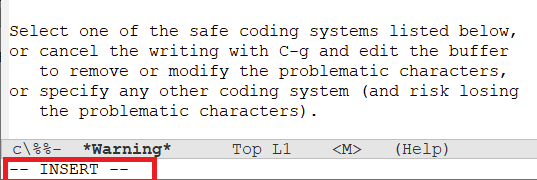
\includegraphics[width=.9\linewidth]{image/13.png}
\end{center}
\end{itemize}
\subsubsection*{5.填写EMACS按键命令}
\label{sec:orgd0ee403}
\begin{table}[htbp]
\caption{基本操作}
\centering
\begin{tabular}{ll}
操作 & 按键\\
\hline
Undo & \textbf{C-\_}\\
Redo & \textbf{C-g}\\
Find file & \textbf{C-x C-f}\\
Save file & \textbf{C-x C-s}\\
Kill buffer & \textbf{C-x C-k}\\
Quit Emacs & \textbf{C-x C-c}\\
Word Command & \textbf{M-x}\\
\end{tabular}
\end{table}

\begin{table}[htbp]
\caption{Org-mode basic command}
\centering
\begin{tabular}{ll}
Operation & Key\\
\hline
local cycle display headline hierarchy & \textbf{Tab}\\
Global cycle display headline hierarchy & \textbf{C-u Tab}\\
Increase level & \textbf{M-left}\\
Decrease level & \textbf{M-right}\\
Move up within level & \textbf{M-up}\\
Move down within level & \textbf{M-down}\\
Move a headline under another top headline & \\
\end{tabular}
\end{table}

\subsubsection*{4. 回答下列问题,并在实验中验证}
\label{sec:org571b624}

\begin{itemize}
\item\relax [N]: \texttt{Normal Mode} [I]: \texttt{Insert Mode} [V]: \texttt{Visual Mode} [C]: \texttt{Command Mode}
\end{itemize}

\begin{table}[htbp]
\caption{VIM Basic Question}
\centering
\begin{tabular}{ll}
Question & Answer (Tips)\\
\hline
switch \texttt{Normal Mode} between \texttt{Visual Mode} & Esc / v\\
switch \texttt{Normal Mode} between \texttt{Insert Mode} & Esc / i\\
which key delete a character [ab \uline{c} de]? & [N]x\\
repeate delete 10 character [ab \uline{cccccccccc} de] & [N]10x\\
delete current line & [N]dd\\
delete line from \uline{t} his point & [N]D\\
Undo & [N]u\\
Redo & [N]C-r\\
move to end of a line & [N]\$\\
move to begin of a line & [N]0\\
move to start of a file & [N]gg\\
move to end of a file & [N]G\\
search in current buffer & [N]/\\
search next / forward & [N]n/N\\
\end{tabular}
\end{table}

\section*{实验二 用 EMACS 的 ORGMODE 编写 WINDBG 实验文档}
\label{sec:org3117558}
\subsection*{一、实验要求}
\label{sec:org38ea837}
\begin{itemize}
\item 熟悉 ORGMODE 语法
\item ORGMODE 插入图片、表格、超级链接的方式
\item 使用第三方插件导出带有 CSS 样式的 html 文件
\item 选做: 将您创建的文档放到 github 上保存并使用 git 命令提交
\item 选做:将放到 github 上生成的 html 文件发布出来,测试是否能远程浏览
\end{itemize}
\subsection*{二、实验要点}
\label{sec:org901dc45}
\subsubsection*{1. 在 ORG 文档中输入以下内容观察 HEADLINE 结构}
\label{sec:org922d01f}
\begin{verbatim}
** Second level
*** Third level
   some text
*** Third level
   more text
\end{verbatim}

\begin{center}
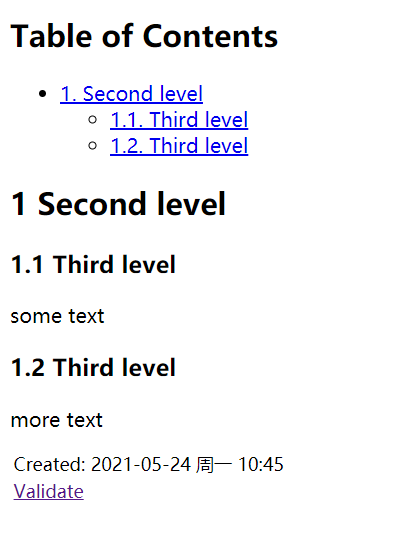
\includegraphics[width=.9\linewidth]{image/14.png}
\end{center}
\subsubsection*{2. 回答以下问题}
\label{sec:orgbe24784}

\begin{table}[htbp]
\caption{Table}
\centering
\begin{tabular}{ll}
Question & Command(Tips)\\
\hline
Create a table in org-mode & Input \texttt{¦ contents ¦ RET}\\
re-align the table without moving the cursor & \texttt{C-c C-c}\\
re-align the table, move to next field & \texttt{TAB}\\
move to previous field & \texttt{S-TAB}\\
re-align the table, move to next row & \texttt{RET}\\
move to beginning/end of field & \texttt{M-a/e}\\
move the current column left & \texttt{M-→/←}\\
kill the current column & \texttt{M-S- ←}\\
insert new column to left of cursor position & \texttt{M-S- →}\\
move the current row up/down & \texttt{M-↑/↓}\\
kill the current row or horizontal line & \texttt{M-S-↑}\\
insert new row above the current row & \texttt{M-S-↓}\\
insert hline below (C-u : above) current row & \texttt{C-c -}\\
insert hline and move to line below it & \texttt{C-c RET}\\
sort lines in region & \texttt{C-c \textasciicircum{}}\\
\end{tabular}
\end{table}

\subsubsection*{3. 插入图片和超级链接}
\label{sec:orgc211dd4}
\href{image/15.png}{这是图片名称,点击此链接在新窗口打开图片}

这是到\href{https://www.baidu.com}{百度}的链接

\begin{center}

\includegraphics[width=.9\linewidth]{image/15.png}
\end{center}


\subsubsection*{4. 用 EMACS 的 ORGMODE 编写 WINDBG 实验文档}
\label{sec:org4e76691}
\begin{itemize}
\item a)实验题目:
\label{sec:orgb78406b}
利用windbg进行虚实地址转换
\item b)实验目的:
\label{sec:org9ab97ec}
利用windbg对内核进行调试,实现虚拟地址向物理地址的转换
\item c)实验环境:
\label{sec:orgc768209}
Windows10;虚拟机Windows7;WinDbg;
\item d)实验内容:
\label{sec:orgd52cd7f}
在配置主机(windows10)下配置WinDbg连接虚拟机中Windows7,进而进行内核调试。
\item e)实验步骤:
\label{sec:org3a2a58e}
\begin{itemize}
\item 1.首先在虚拟机中创建一个文档,里面输入“hello!lge”
\begin{center}
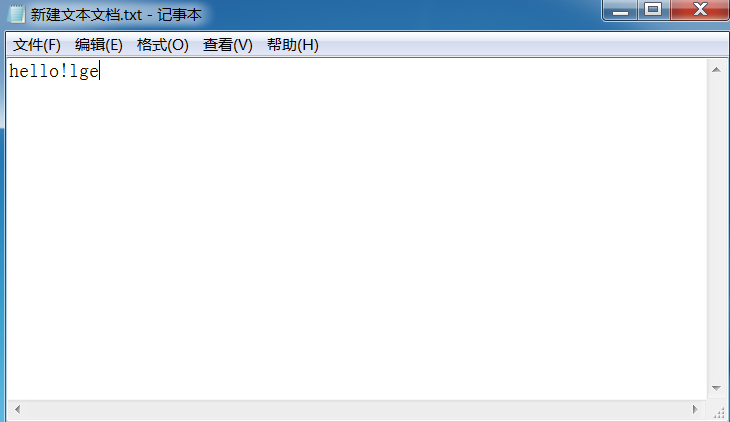
\includegraphics[width=.9\linewidth]{image/16.png}
\end{center}
\item 2.使用windbg连接虚拟机进行内核调试,查找notepad.exe进程,可以看到进程块起始地址
\begin{center}
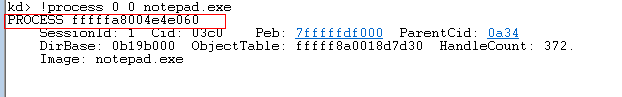
\includegraphics[width=.9\linewidth]{image/17.png}
\end{center}
\item 3.使用下面命令,然后再输入g命令将Windbg当前调试进程切换到notepad.exe
\begin{center}
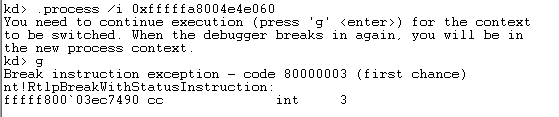
\includegraphics[width=.9\linewidth]{image/18.png}
\end{center}

\item 4.可以看到cr3的内容已经发生改变
\begin{center}
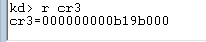
\includegraphics[width=.9\linewidth]{image/19.png}
\end{center}
\item 5.查找notepad中字符串所在的虚拟地址位置
\begin{center}
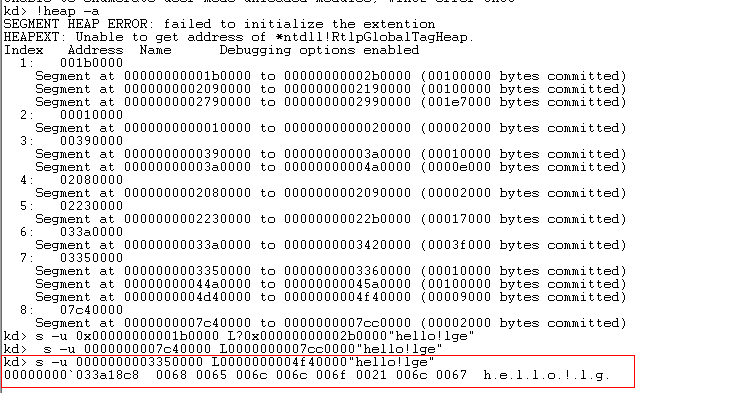
\includegraphics[width=.9\linewidth]{image/20.png}
\end{center}
\item 6.测试是否正确,发现是自己写进去的字符串。
\begin{center}
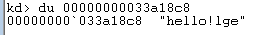
\includegraphics[width=.9\linewidth]{image/21.png}
\end{center}
\item 7.将虚拟地址的十六进制转换为2进制
\begin{center}
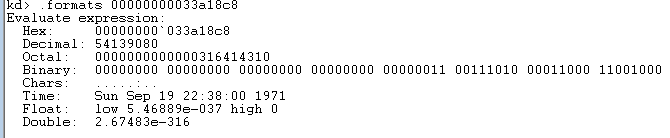
\includegraphics[width=.9\linewidth]{image/22.png}
\end{center}
\item 8.可以发现:
\end{itemize}
\begin{verse}
PML4E索引:0000 0000=x0\\
PDPTE索引:0000 0000=0x0\\
PDE索引:0011 0011 = 0x19\\
PTE索引:11010 0001 = 0x1a1\\
页内偏移:1000 1100 1000 = 0x8c8\\
\end{verse}
\begin{itemize}
\item 9.目标进程的DirBase为0xb19b000, PML4E索引为0,所以目的地址为:0xb19b000.
\begin{center}
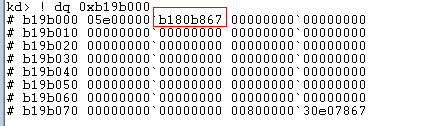
\includegraphics[width=.9\linewidth]{image/23.png}
\end{center}
\item 10.因为PDPTE索引为0,所以目的地址为0xb180b000
\begin{center}
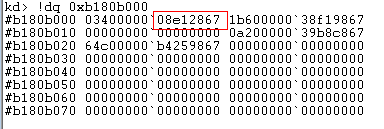
\includegraphics[width=.9\linewidth]{image/24.png}
\end{center}
\item 11.PDE索引为0x19,所以要加上,目的地址为:0x8e12000+0x19*8
\begin{center}
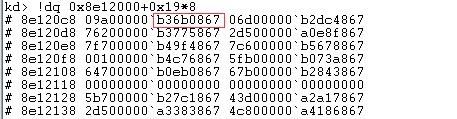
\includegraphics[width=.9\linewidth]{image/25.png}
\end{center}
\item 12.PTE索引为0x1a1,所以要加上0x1a1*8,目的地址为:0xb36b0000+0x1a1*8
\begin{center}
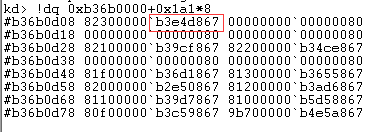
\includegraphics[width=.9\linewidth]{image/26.png}
\end{center}
\item 13.页内偏移为0x8c8,索引在0xb3e4d000的基础上加上偏移值就是目的地址。可以看到我们在程序中输入的字符串。
\begin{center}
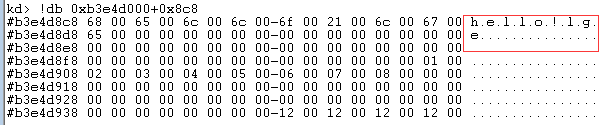
\includegraphics[width=.9\linewidth]{image/27.png}
\end{center}
\end{itemize}
\end{itemize}
\subsubsection*{5. 选做:将导出的 html 文档发布到 github 上}
\label{sec:org5a692e3}
\begin{itemize}
\item a) 将文档保存到 github
\label{sec:org303a2a2}
\item b) 将导出的 html 进行发布
\label{sec:orgbc3904d}
\end{itemize}
\end{document}
